%%%%%%%%%%%%%%%%%%%%%%%%%%%%%%%%%%%%%%%%%%%%%%%%%%%%%%%%%%%%%%%%%%%%%%%
%% Vorlage f�r Abschlussarbeiten                                     %%
%%-------------------------------------------------------------------%%
%% Datei:        appendix.tex                                        %%
%% Beschreibung: Weitere Informationen, Schaltpl�ne und Quelltext    %%
%% Autor: 			 Stefan Herrmann                                     %%
%% Datum:        03.12.2012                                          %%
%% Version:      1.0.1                                               %%
%%%%%%%%%%%%%%%%%%%%%%%%%%%%%%%%%%%%%%%%%%%%%%%%%%%%%%%%%%%%%%%%%%%%%%%

\chapter{Anhang}
\index{Anhang}
In den Anhang kommen alle entworfenen und umgesetzten Schaltpl�ne\index{Schaltplan}, Layouts etc., die wichtig f�r die Arbeit sind. Alle Anh�nge sollten aus dem Text heraus referenziert werden. Auch hier im Anhang k�nnen Unterkapitel eingef�gt werden.
\newpage

\section{Schaltpl�ne}
\index{Schaltpl�ne}
Wenn Schaltpl�ne bzw. Layouts eingef�gt werden, dann sind immer die Kenndaten mit aufzuf�hren. Hierzu geh�ren der Platinen-Name\index{Platine}, die Platinen-Nummer\index{Platinen-Nummer}, die Version\index{Version}, der Status und ob noch Fehler und �nderungen offen sind.

\newpage

\begin{figure}[H]
	\centering
		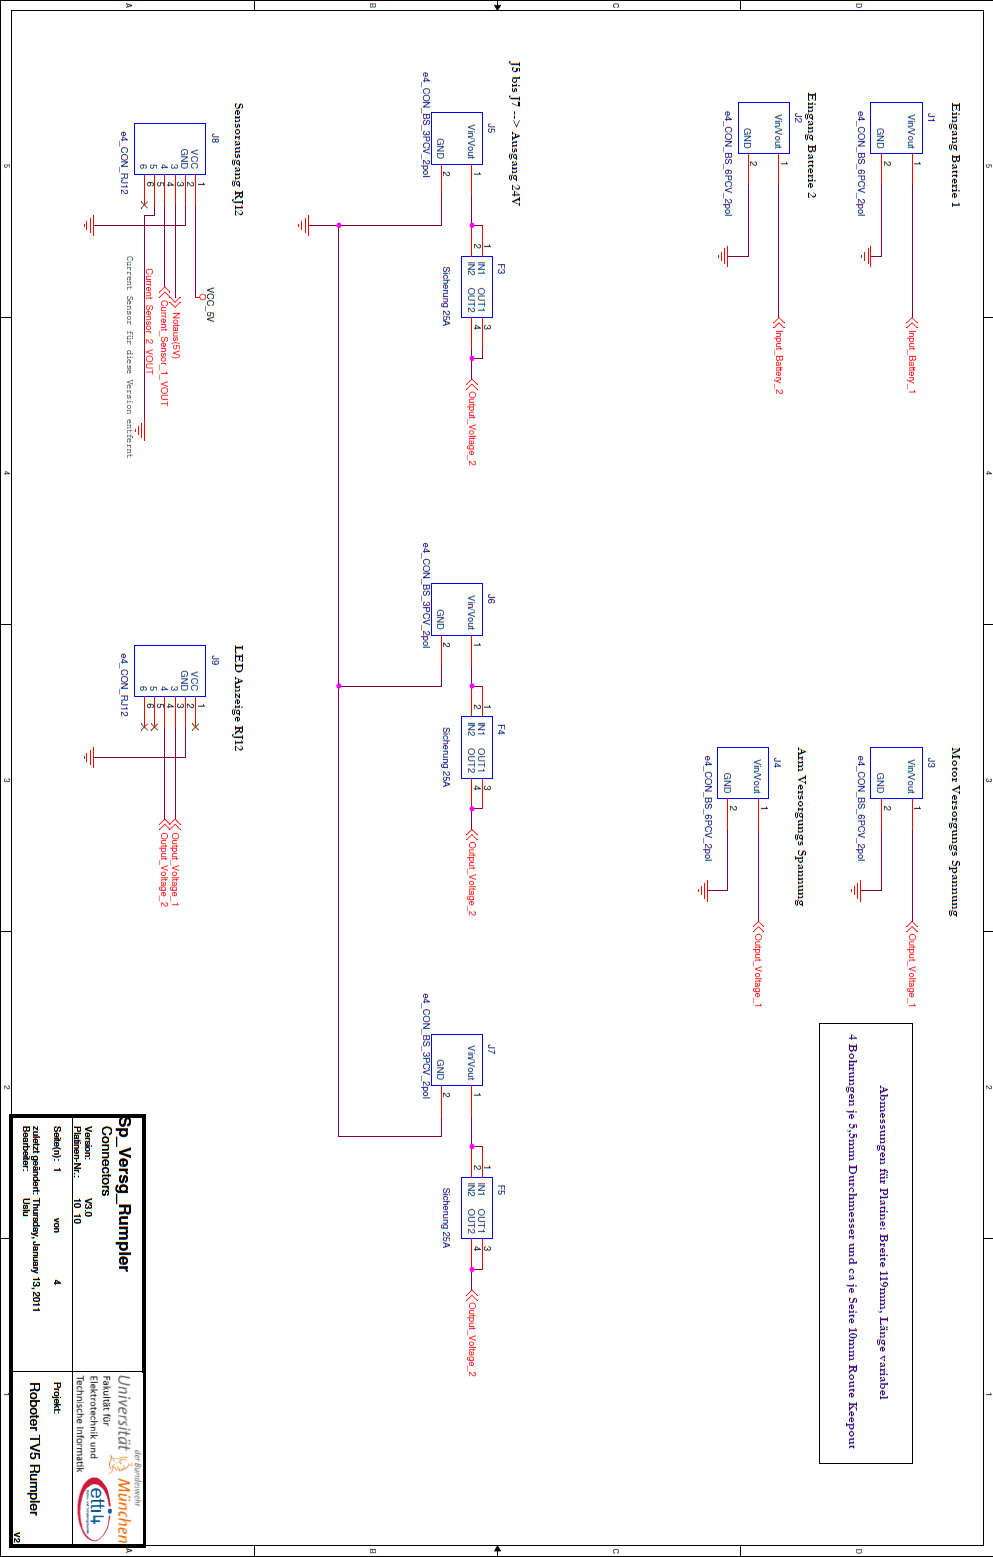
\includegraphics[width=0.8\textwidth]{images/appendix/Design01.png}
	\caption{Schaltungsdesign f�r die Spannungsversorgungsplatine}
	\label{fig:Design01}
\end{figure}


\begin{figure}[H]
	\centering
		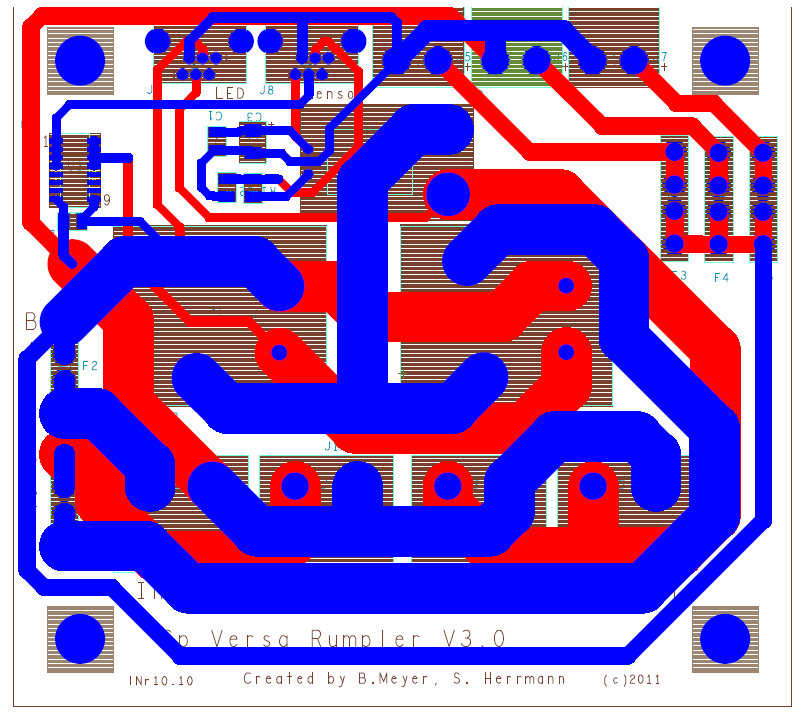
\includegraphics[width=0.8\textwidth]{images/appendix/layout.png}
	\caption{Layout f�r die Spannungsversorgungsplatine.}
	\label{fig:layout}
\end{figure}

\newpage

\section{Projektplan mit themenbezogenem Zeitaufwand}
\index{Projektplan}\index{Zeitaufwand}\index{Aufwand}
Am Anfang der Arbeit sollte man sich Gedanken dar�ber machen, welche Arbeiten notwendig sind und wie viel Zeit man hierf�r ben�tigt. Au�erdem sollte eine �bersicht �ber die tats�chlich aufgewendeten Stunden erstellt werden. Die Planung der Arbeit kann �ber ein GANTT-Diagramm\index{GANTT-Diagramm} erfolgen. Um den Aufwand f�r bestimmte T�tigkeiten zu bestimmen, k�nnen die Mitarbeiter des Instituts~4 befragt werden. 

\begin{figure}[H]
	\centering
		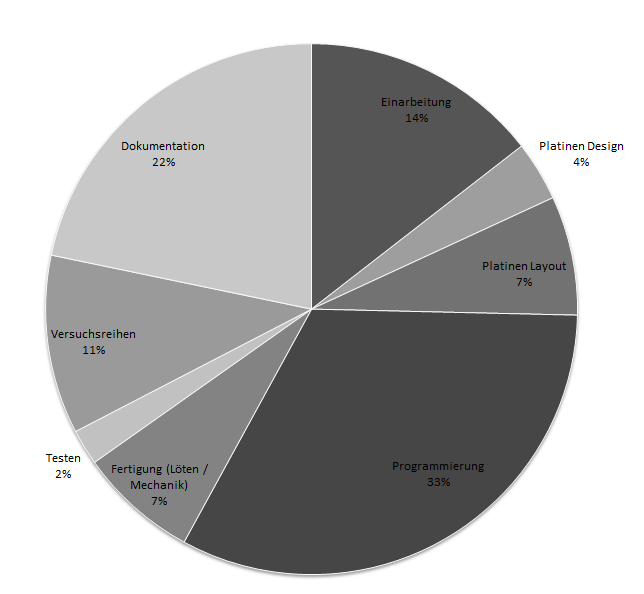
\includegraphics[width=0.8\textwidth]{images/appendix/arbeitsaufwand.png}
	\caption{Themenbezogene Stundenaufschl�sselung f�r die Abschlussarbeit.}
	\label{fig:arbeitsaufwand}
\end{figure}


\begin{figure}[H]
	\centering
		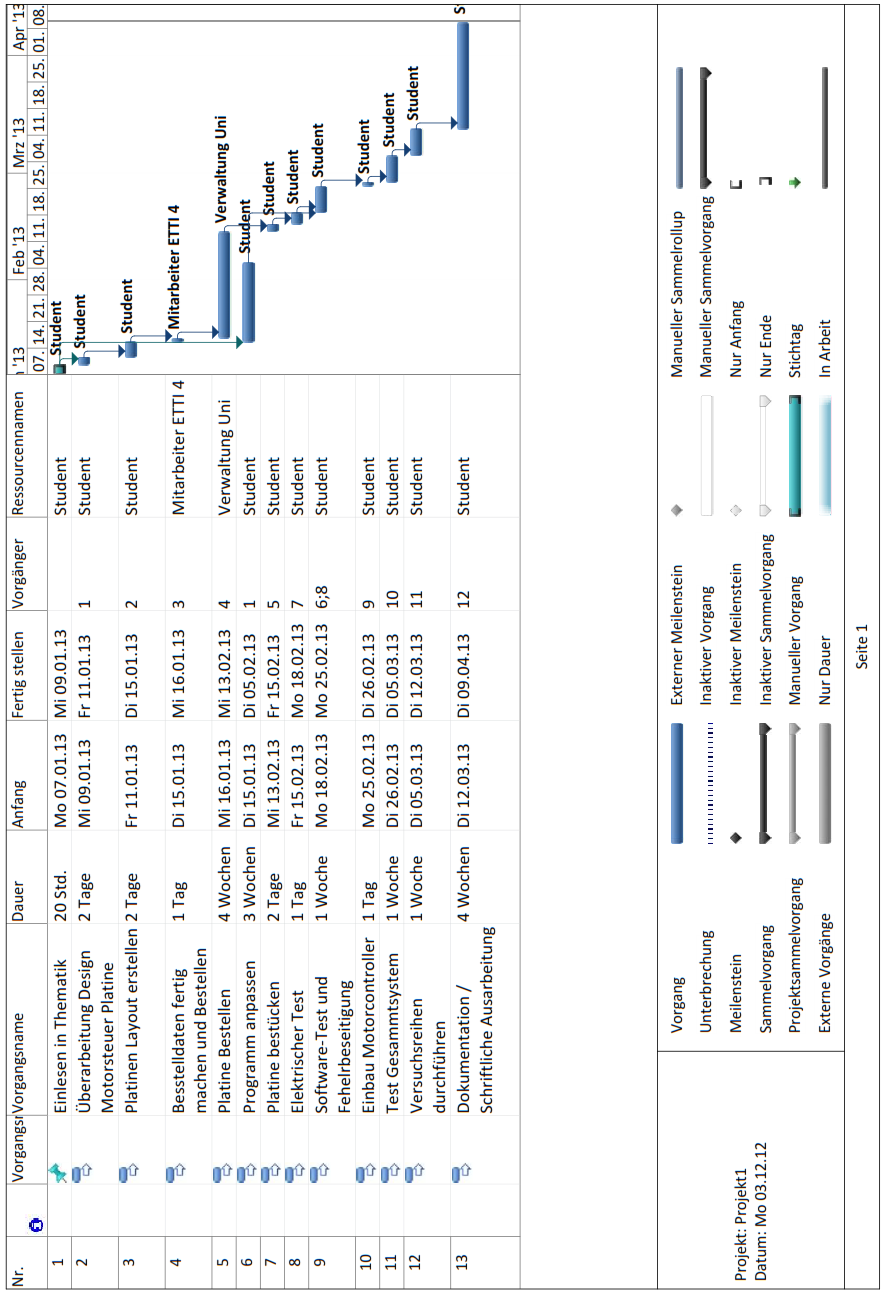
\includegraphics[width=0.8\textwidth]{images/appendix/projektplan.png}
	\caption{Aufgaben�bersicht f�r die Abschlussarbeit.}
	\label{fig:projektplan}
\end{figure}




